\documentclass[11pt,a4paper]{article}
\usepackage[margin=25mm]{geometry}
\usepackage{iftex}
\ifPDFTeX\usepackage[T1]{fontenc}\usepackage[utf8]{inputenc}\fi
\usepackage{amsmath,amssymb,graphicx,booktabs,array}
\usepackage[authoryear,round]{natbib}
\usepackage{caption,placeins}
\usepackage[unicode,breaklinks=true,hidelinks]{hyperref}
\setlength{\parindent}{0pt}\setlength{\parskip}{5pt}
\setlength{\emergencystretch}{3em}\setlength{\tabcolsep}{3pt}
\clubpenalty=10000\widowpenalty=10000
\captionsetup{font=small,labelfont=bf}
\newcounter{proposition}
\begin{document}
\begin{center}\Large\bfseries Hard to Beat: Historical Rules versus Conditional Quantile Models for Peak Net-Position Limits\end{center}

\begin{abstract}Dealers monitor the largest absolute position reached before a review horizon ends. We compare conditional quantile models with historical rules using hourly FX positions, weekly New York Fed positions and dealer aggregates in 17 CFTC futures markets. Histories and update schedules are matched. Historical rules are hard to beat. First, FX regression lowers matched loss by 14.8\% and 16.6\% across two periods, but its ranking against a shorter rolling rule changes. Second, historical rules beat regression in 34 of 48 New York Fed comparisons and 29 of 34 CFTC comparisons. They usually remain in the model confidence set alongside alternatives. In calibrated simulations, expanding the penalty menu cuts the constant-parameter median excess loss from 116.2\% to near zero; the registered switching increment is unsupported. Third, in CFTC, lower scores need not mean lower limit costs: higher reserve charges and lower fixed breach charges generally favor expanded regression. The evidence is retrospective, and the original FX evaluation period had been inspected beforehand.\end{abstract}

\noindent\textbf{Keywords:} Peak net positions; Quantile forecasting; Historical benchmarks; Forecast comparison; Calibration; Dealer positions.\par\medskip

\section{Introduction}\label{sec:intro}

Dealer position limits concern the largest exposure reached before a review horizon ends. A position can finish within its limit after crossing it earlier (Figure~\ref{fig:example}). We compare historical and conditional forecasts of this sampled absolute-position peak.

Historical headroom combines the current position with completed past peak behavior. Conditional models estimate additional relationships from finite historical windows. Matched histories and update schedules show whether the added conditioning improves the forecast.

\begin{figure}[htbp]\centering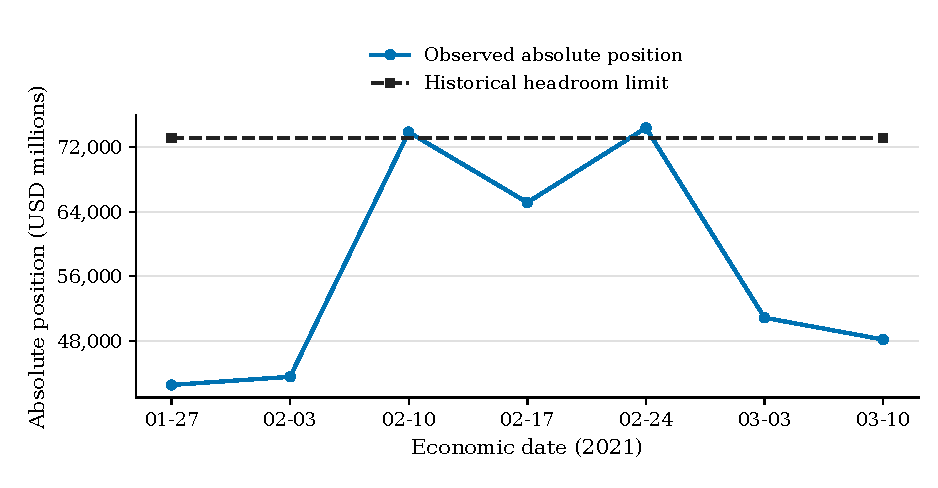
\includegraphics[width=.94\linewidth]{figures/v9-endpoint-peak-example.pdf}
\caption{A selected Treasury-bill path whose endpoint returns within the historical report after an intervening breach. The rule chooses the earliest eligible original evaluation window. Endpoint containment can conceal a peak breach.}\label{fig:example}
\end{figure}

Our evidence covers hourly FX positions, their daily aggregates, New York Fed categories and CFTC dealer-category futures. The two official weekly systems report different aggregate exposures. Original protocol comparisons retain their original reference procedures and values.

Three questions organize the evaluation.

\textbf{RQ1} asks whether conditional quantile methods improve sampled peak forecasts with matched histories and update schedules.

\textbf{RQ2} asks whether those gains extend across frequencies and independently reported dealer-position aggregates.

\textbf{RQ3} asks whether score gains imply lower limit costs under reserve, breach and exceedance preferences.

The paper makes three empirical findings.

\textit{First, matched FX gains recur, but rankings against a shorter rolling rule change.} The period comparisons separate conditioning gains from the reference procedure (Table~\ref{tab:fx}). Delayed calibration preserves the later matched gain while changing breach behavior.

\textit{Second, historical rules remain competitive in weekly data, and penalty menus explain large losses in the calibrated simulations.} The panel and independent CFTC reporting system favor historical controls in most comparisons (Tables~\ref{tab:weekly} and~\ref{tab:v10-cftc-contracts}). Historical procedures usually remain in model confidence sets alongside alternatives (Table~\ref{tab:v10-mcs-main}). Expanding the simulation menu brings short-history full regression close to its historical reference; the registered switching increment is unsupported.

\textit{Third, higher reserve charges and lower fixed breach charges generally favor expanded regression in CFTC.} The direction has local exceptions (Figure~\ref{fig:v10-cost}). Lower scores therefore need not mean lower limit costs, and validation should report reserve amounts, breach counts and exceedance amounts together.

Section~\ref{sec:target} defines the response. Section~\ref{sec:results} answers RQ1 and RQ2; Section~\ref{sec:cost} answers RQ3. Elementary floor and endpoint properties support the forecast definitions. The forecasting, comparison and cost-accounting methods are established.

\FloatBarrier

\section{Related literature}\label{sec:literature}

Wisniewski and colleagues forecast signed next-hour position intervals using historical states, calendar information and local prediction methods \citep{wisniewski2020,wisniewski2024}. Their chronological training, calibration and test design reports scores and coverage together. The present peak response uses a complete future path segment and the current magnitude, producing different labels and limits.


Path-risk forecasts address within-period extremes. MaxVaR studies the worst cumulative portfolio return under fixed holdings and diffusion assumptions \citep{boudoukh2004}. The payment-liquidity thesis forecasts conditional maximum deficits from confidential transactions \citep{hoogen2017}. Settlement studies examine tail liquidity needs and collateral requirements \citep{petrunia2019,arjani2020}. Duffie and colleagues study dealer capacity and Treasury-market functioning, including PnL quantile forecasts \citep{duffie2023}. These responses differ from the sampled absolute-position peak.


Regression quantiles target asymmetric forecast errors directly \citep{koenker1978}. Autoregressive quantiles and quantile forests supply other conditioning structures \citep{engle2004,meinshausen2006}. Consistent scores and elementary-score representations permit comparison across evaluation preferences \citep{gneiting2011,ehm2016}. Table~\ref{tab:literature} locates the present peak response, completed labels and matched historical controls.


\begin{table}[htbp]\centering\footnotesize\uchyph=1\hyphenation{con-fi-den-tial con-di-tion-al re-gres-sion com-plet-ed el-e-men-ta-ry ex-pand-ing}
\caption{Closest literature and the peak-position task. A dash marks a dimension unverified in the consulted passage. Established methods support the comparison of a common peak response.}\label{tab:literature}
\begin{tabular}{>{\raggedright\arraybackslash}p{2.4cm}>{\raggedright\arraybackslash}p{2.1cm}>{\raggedright\arraybackslash}p{1.5cm}>{\raggedright\arraybackslash}p{1.6cm}>{\raggedright\arraybackslash}p{1.6cm}>{\raggedright\arraybackslash}p{1.7cm}>{\raggedright\arraybackslash}p{1.7cm}}\toprule
Study & Response & Data unit & Peak floor & Label timing & Evaluation & Source scope\\\midrule
\shortstack[l]{Wisniewski\\et al. (2020)} & Signed endpoint interval & One FX market maker & --- & Ordered train/\allowbreak calibrate/\allowbreak test & Scores and hit tests & One source family\\
\shortstack[l]{Boudoukh\\et al. (2004)} & Worst portfolio return & Stylized fixed portfolio & Different initial-value anchor & Analytic diffusion & Tail ratios and monitoring & Parameter cases\\
\shortstack[l]{van den\\Hoogen (2017)} & Cumulative payment-deficit peak & Con\-fi\-den\-tial bank payments & Absolute-position floor --- & Path simulation & EVT methodology; results partly confidential & Bank payment task\\
\shortstack[l]{Duffie\\et al. (2023)} & Capacity, illiquidity, PnL quantiles & Dealer/\allowbreak market sources & --- & Expanding PnL fits & Capacity and PnL forecasts & Several sources\\
\shortstack[l]{Engle and\\Manganelli\\(2004)} & Return quantile & Asset returns & --- & Lagged predictors & Quantile scores and DQ & Several returns\\
\shortstack[l]{Ehm et al.\\(2016)} & Quantile/\allowbreak expectile comparison & Multiple forecast examples & --- & Original example designs & El\-e\-men\-tary-score curves & Multiple tasks\\
\shortstack[l]{Meinshausen\\(2006)} & Conditional response quantile & Regression examples & --- & Original regression splits & Conditional distributions & Several datasets\\
This study & Sampled absolute-position peak & FX record; weekly\allowbreak{} totals & Observed current magnitude & Completed forward labels & Scores, breaches, MCS, costs & Related aggregate tasks\\
\bottomrule\end{tabular}
\par\smallskip\begin{minipage}{.98\linewidth}\footnotesize The payment-thesis reading is partial. Dashes mark unverified dimensions in the consulted passages; shared source lineage leaves input-byte identity unverified.\end{minipage}
\end{table}

The matched FX gain changes interpretation with its reference. Weekly historical controls remain competitive, while expanded simulation menus remove the large short-history loss and leave the registered switching increment unsupported. In CFTC, higher reserve and lower fixed breach charges generally favor regression, with local exceptions. Established forecast tests support the comparisons \citep{dm1995,gw2006,mcs2011}. Inventory-sensitive quoting motivates exposure monitoring \citep{avellaneda2008}; here, the forecasts are scored on observed paths.

\FloatBarrier

\section{The forecast target}\label{sec:target}

The target is the largest sampled absolute position from issue time through the stated horizon. Let \(N_t\) denote signed position and \(\mathcal F_t\) the issue-time information. The peak \(Y_{t,H}\), observed floor \(B_t\) and nonnegative headroom \(Z_{t,H}\) satisfy the following identities.


\[
Y_{t,H}=\max_{0\le h\le H}|N_{t+h}|,\qquad B_t=|N_t|,\qquad Z_{t,H}=Y_{t,H}-B_t\ge0.
\]

A feasible limit covers the current observed exposure. Figure~\ref{fig:example} shows an endpoint inside the historical report after an earlier breach. We score reports with pinball loss and count a strict breach when the peak exceeds the limit.


\[
\rho_\tau(u)=\tau u_+ +(1-\tau)(-u)_+,\qquad I_{t,H}=\mathbf 1\{Y_{t,H}>C_{t,H}\}.
\]

\refstepcounter{proposition}\noindent\textbf{Proposition~\theproposition{} (known-floor projection).}\label{prop:floor} Suppose \(Y\ge B\) almost surely and the issue information contains \(B\). Projecting any forecast \(c\) to \(\max\{B,c\}\) weakly improves pinball loss for every possible outcome, with an exact gain below the floor. If \(q\) is the true conditional lower inverse quantile at level \(1-\alpha\), its strict exceedance probability is at most \(\alpha\). At an atom of the response distribution, that probability can be smaller than the nominal tail probability.


\[
\rho_\tau(Y-c)-\rho_\tau(Y-\max\{B,c\})=\tau(B-c)_+,\qquad \Pr(Y>q\mid\mathcal F_t)\le\alpha.
\]

\refstepcounter{proposition}\noindent\textbf{Proposition~\theproposition{} (classical endpoint-to-peak bound).}\label{prop:levy} Let future increments be independent and individually symmetric about zero, with partial sums \(S_h\). Fix a starting position \(x\), set \(B=|x|\), and let \(q\) be the population \((1-\alpha/2)\) quantile of \(|S_H|\). The triangle inequality and the classical scalar L\'evy maximal inequality then imply the following bound, including strict inequalities at atoms \citep{sussman2023}. Neither identical increment distributions nor finite increment moments are required for this population statement.


\[
\Pr\!\left(\max_{0\le h\le H}|x+S_h|>B+q\right)\le\Pr\!\left(\max_h|S_h|>q\right)\le2\Pr(|S_H|>q)\le\alpha.
\]

Supplement Sections S1--S2 prove both statements and distinguish population quantiles from their empirical plug-ins; Sections S3--S5 give the bound simulations. A conditional application requires independence, symmetry and the stated endpoint quantile under the law given issue information. The separate bound simulations distinguish mean-reverting levels from serially correlated increments.


Separately fitted horizon forecasts can violate the ordering of true peak quantiles. Short-history FX regression crosses across horizons on 640 evaluation origins. Label nesting, floor coverage and strict-breach definitions provide additional checks on the issued reports.


\FloatBarrier

\section{Data}\label{sec:data}

The FX application uses the hourly Net Position Time Series Dataset, reporting market-maker client-flow positions \citep{dataset,wisniewski2020}. It contains 18,576 records in source USD units. The later, earlier and full-prefix comparisons use distinct chronological issue grids and the same sampled-peak definition.

The weekly data are New York Fed Primary Dealer Statistics \citep{nyfeddata}. Reporting definitions follow the government-securities dealer framework and position-accounting instructions \citep{fr2004_2013,fr2004_2024}. The Treasury-bill series has 706 economic-date observations in USD millions. The values are fair-value positions aggregated as long-minus-short totals. Additional categories pass metadata and calendar checks and use complete weekly grids, with separate fits by category.

Daily aggregation takes the last recorded position on each nonempty source-naive calendar day. It retains partial boundary days, yielding 930 days and 501 common evaluation issues. Reports use the completed day's end as their issue clock. The resulting target is a peak over subsequent daily records.

The CFTC application is a retrospective survivor-universe, economic-date replay. It uses futures-only Dealer/Intermediary long positions minus short positions \citep{cftcTFF}. The fixed screen requires uninterrupted report weeks from 2010, stable literal codes, exchange and units. It excludes documented consolidation-code families before ranking eligible contracts by full-sample mean open interest. Seventeen contracts qualify, fewer than the planned maximum of twenty. Supplement Section S30 lists every selected code and explains the eligibility rules; complete code-level exclusions remain linked there.

There are 877 weekly positions through 20 October 2026. Validation uses 52 origins; evaluation uses the last 260 eligible origins with horizon six. The evaluation position dates run from 21 September 2021 to 8 September 2026. Its final peak label completes on 20 October 2026. Refit frequency is thirteen records; histories are 52 and 260. Positions usually refer to Tuesday and are released Friday; this application replays downloaded economic dates.

Every method within a comparison uses identical peak labels, current floors and issue origins. Source units and histories remain distinct across series. The same-record aggregation holds dealer identity fixed while changing the measurement clock.

\FloatBarrier

\section{Forecasting methods}\label{sec:methods}

Forecasts target the conditional quantile at \(\tau=19/20\). The horizons \(H\in\{6,24\}\) count subsequent source records, and each peak includes the issue position. Calendar gaps extend an FX horizon's elapsed span; weekly and daily steps represent different review intervals. The nineteen-to-one error-weight preference defines the evaluation score.

Historical headroom uses the corrected empirical rank of completed headrooms and adds its report to the current magnitude. Translated paths reanchor historical signed paths, while historical-peak quantiles are projected to the observed floor. The endpoint plug-in uses an absolute-displacement quantile; Table~\ref{tab:methods} gives the executed menus and schedules.

Ridge quantile regression links mature headroom to issue-known position states and calendar variables. The larger set contains 33 predictors plus an unpenalized intercept. The four-predictor variant uses current magnitude, signed level and two increment RMS measures. All standardization uses mature training observations. Expanded-menu full regression changes only the penalty grid.

Local quantiles use neighboring historical states, with an increment-scaled variant. Filtered paths simulate positions from GARCH-standardized empirical innovations drawn independently with replacement \citep{hull1998,barone1999}. Quantile forests use leaf distributions; tail methods fit volatility-scaled headroom \citep{meinshausen2006,mcneilfrey2000}. Supplement Sections S7 and S11--S18 report benchmark results and failures; Section S34 links the complete legacy inventories.

Further comparisons apply delayed calibration, fixed combinations and conservative selection to the same peak response. A headroom CAViaR recursion and calibration wrappers follow existing methods \citep{engle2004,gibbs2021}. Calibration parameters update after outcomes mature. Fixed mean and median combinations use predefined members. Conservative selection favors the strongest shrinkage within one paired HAC standard error of the validation winner. This adapts one-standard-error selection \citep{hastie2009} to paired forecast losses.

\begin{table}[htbp]\centering\small
\caption{Forecast definitions and executed menus. Codes occur here to connect with the result files. Matched histories and update schedules make the reference explicit.}\label{tab:methods}
\begin{tabular}{>{\raggedright\arraybackslash}p{2.9cm}>{\raggedright\arraybackslash}p{6.0cm}>{\raggedright\arraybackslash}p{5.3cm}}\toprule
Method & Forecast definition & Executed menu / setting\\\midrule
Historical headroom (F) & Current floor plus a quantile of completed peak headrooms & FX histories \{720,2880\}; weekly \{52,260\}\\
Translated path (S) & Translate completed signed paths to the current position before taking their peaks & Same completed-label pools; fixed-window and rolling-window controls\\
Historical peak (K) & Historical absolute-peak quantile projected to the current floor & Same histories and update controls\\
Quantile regression (QR) & Training-scaled headroom regression with ridge slopes and an unpenalized intercept & Original three-point menu; six-point menu $\{0.001,0.01,0.1,1,10,\infty\}$\\
Local quantiles (KNN) & Neighbor headroom quantile, with a separate increment-scale variant & Training-only transforms and fixed neighbor menus; Supplement Sections S8 and S23\\
Parsimonious regression (QR4) & Current signed/magnitude positions and short/long increment RMS & Original five-point menu; six-point paired comparison below\\
Endpoint plug-in (L) & Floor plus a high absolute-displacement endpoint quantile & Proposition~\ref{prop:levy}; empirical plug-in evaluated separately\\
Further benchmarks & Autoregressive replay; filtered paths; peak-tail fit; quantile forest & Existing bounded specifications; results and complete failures linked from Supplement Sections S7 and S34\\
Coverage and combinations & Delayed projected ACI-style wrappers; headroom SAV; fixed forecast combinations & Original-source wrapper/SAV inventory and broader combination inventory are separate\\
\bottomrule\end{tabular}
\par\smallskip\begin{minipage}{.98\linewidth}\footnotesize Training histories count completed labels. Fixed-window models refit every 24 FX records or 13 weekly records. Quantile and normalization conventions are detailed in Supplement Sections S8 and S23; this table retains the executed menus.\end{minipage}
\end{table}

\FloatBarrier

\section{Evaluation design}\label{sec:evaluation}

At refit \(r\), training labels are eligible only when \(i+H\le r\). Predictors use issue-known observations, and training transforms remain fixed until the next refit. Original comparisons select parameters in the preceding validation segment. The full-prefix backcast holds its specified penalties fixed. Weekly selection uses 52 outer validation origins with overlapping labels.

Matched comparisons fix completed-response history and refit schedule for regression and historical headroom. The main FX reference uses a shorter rolling history. The main Treasury reference shares regression's longer history and refit schedule. Tables~\ref{tab:fx} and~\ref{tab:weekly} report both alongside the other comparison sets.

Accuracy uses mean pinball loss; breaches are strict peak exceedances. Evaluation scores passive reports on the observed position paths. Paired loss differences use HAC covariance with the horizon-based bandwidth rule \citep{dm1995,nw1987}. Tables identify the small-sample adjustment and named multiplicity families \citep{hln1997,holm1979}. Hit diagnostics use a fixed spaced grid and condition the transition likelihood on its initial hit \citep{kupiec1995,christ1998}.

\subsection{Research design and transparency}

The original protocol fixes the two main comparisons and their reference procedures. Other p-values are exploratory and unadjusted unless stated. Supplement Sections S14--S17, S19, S23 and S29--S34 give comparison families, chronology and failure inventories. The new studies retain separate estimation, simulation and reporting records. Menu design follows the earlier simulation results but precedes paired computations. CFTC design precedes acquisition; two format clarifications precede all forecasts. MCS and cost specifications lock before calculations on previously inspected reports. These are frozen descriptive decision rules within a retrospective research program.

\subsection{Multiple-method forecast comparison}

We form a 90\% model confidence set separately for each complete source, period, horizon and history grid \citep{mcs2011}. The range statistic uses 1,000 stationary-bootstrap replications in arch 8.0.0. Block length is $\max\{H,\lceil n^{1/3}\rceil\}$. All complete saved procedures enter; incomplete prior methods remain explicitly unavailable. Entire origin grids and targets must match. The nominal level presumes suitable loss dependence; it does not adjust earlier research-stage model development.

Exact duplicate loss columns enter the bootstrap once and their procedure labels are unfolded afterward. Matched F/I aliases merge only after full forecast and target equality. Rolling references remain distinct. Literal sole membership differs from a sole surviving loss class containing several procedures. The fractions summarize related tasks, with no independent cross-market pooled test.

\FloatBarrier

\section{Results}\label{sec:results}

\subsection{RQ1: matched accuracy and reference stability}

Long-history FX regression beats matched historical headroom in both periods. Table~\ref{tab:fx} separates these matched controls from the shorter rolling reference, whose earlier-period ranking reverses.

Delayed calibration retains the later matched FX gain. Its breach count remains slightly higher than wrapped historical headroom on common origins (Table~\ref{tab:fx}).

Supplement Sections S20--S21 and S26 report the state, target-level and overlapping full-prefix comparisons (Tables S19--S21 and S25--S26). Full-prefix regression lowers matched loss by 12.2\% but records 416 versus 282 breaches. Its rolling-reference DM p-value is 0.055. Longer-horizon gains coexist with reference-sensitive losses in the complete tables.

\begin{table}[htbp]\centering\small
\caption{Long-history short-horizon FX regression under two references and periods. Negative percentages favor regression. Matched gains recur while the rolling-reference direction changes.}\label{tab:fx}
\begin{tabular}{>{\raggedright\arraybackslash}p{2.6cm}>{\raggedright\arraybackslash}p{4.4cm}>{\raggedleft\arraybackslash}p{2.5cm}>{\raggedleft\arraybackslash}p{1.5cm}>{\raggedright\arraybackslash}p{3.2cm}}\toprule
Period / procedure & Reference & Loss change (\%) & Issues & Strict breaches (regression / reference)\\\midrule
Later / original main comparison & Shorter-history rolling headroom & -12.66 & 6625 & 376 / 332\\
Later / matched & Same-history fixed-window headroom & -14.77 & 6625 & 376 / 360\\
Earlier / original structure & Shorter-history rolling headroom & +3.17 & 1440 & See complete earlier-period tables\\
Earlier / matched & Same-history fixed-window headroom & -16.62 & 1440 & 20 / 16\\
Later / coverage-wrapped & Same-history wrapped headroom & -15.00 & 6625 & 329 / 328\\
\bottomrule\end{tabular}
\par\smallskip\begin{minipage}{.98\linewidth}\footnotesize Regression uses history 2880 and horizon 6; the original rolling reference uses 720. The earlier matched comparison is the original three-penalty regression, not the later one-standard-error selection rule. The wrapper comparison is a separate finite projected delayed ACI-style exercise.\end{minipage}
\end{table}

\subsection{RQ2: daily, weekly and independently reported positions}

The reference-sensitive hourly results motivate comparisons with other measurement clocks and reporting systems. These comparisons retain their own matched histories and completed peak labels.

Beyond the matched long-history case, short-history FX regression performs poorly at the longer horizon. Loss rises by 31.5\% against matched historical headroom. Regression records 924 breaches against 427 for the reference; the full horizon map retains the other adverse comparisons.

At weekly frequency, the Treasury-bill comparison also favors historical headroom on accuracy and breaches. The earlier short-window version has a different history and retains its separate adverse result (Table~\ref{tab:weekly}).

Stronger regularization narrows weekly panel losses but leaves historical rules ahead (Table~\ref{tab:weekly}). Conservative selection chooses the intercept-only report in 17 of 26 earlier weekly cells. Its worst loss remains the Treasury-bill short-window, 24-step comparison, despite the conservative selection rule.

Simpler conditional reports and fixed combinations also give mixed weekly results. The median combination lowers Treasury-bill loss by 4.0\%, while the mean combination raises it by 2.8\%. The headroom recursion is also worse. Supplement Sections S16--S18 retain the combination and headroom-recursion results, including completed losses and failures (Tables S14--S17).

Returning to the same FX record, historical headroom wins seven of eight daily comparisons. The exception uses four predictors, history 260 and horizon 6, reducing loss by 3.0\%. It records 37 breaches versus 30 for matched headroom. Daily aggregation therefore preserves the score--breach disagreement while changing the leading forecast in most comparisons.

\begin{table}[htbp]\centering\small
\caption{Weekly evidence across the original main comparison, added panel and earlier-period comparisons. Counts refer to related tasks rather than independent dealers. Stronger regularization narrows losses while leaving substantial failures.}\label{tab:weekly}
\begin{tabular}{>{\raggedright\arraybackslash}p{4.3cm}>{\raggedright\arraybackslash}p{4.7cm}>{\raggedleft\arraybackslash}p{2.7cm}>{\raggedright\arraybackslash}p{2.5cm}}\toprule
Comparison set & Procedure & Loss change / median (\%) & Higher-loss cells\\\midrule
Original Treasury-bill main comparison & Original regression, long history & +50.79 & Original main comparison\\
Earlier Treasury-bill short-window version & Short-history short-window version & +144.30 & Different history\\
Additional panel & Original full regression & +92.63 & 45 / 48\\
Additional panel & Four-predictor regression & +9.91 & 37 / 48\\
Additional panel & Full regression, expanded penalties & +9.22 & 34 / 48\\
Additional panel & Ordinary empirical headroom quantile & +0.50 & 30 / 48\\
Earlier weekly groups & Validation-minimum expanded rule & +4.15 & 26 groups\\
Earlier weekly groups & One-standard-error rule & +5.37 & 26 groups\\
\bottomrule\end{tabular}
\par\smallskip\begin{minipage}{.98\linewidth}\footnotesize The original bill main comparison has 54 versus 28 strict breaches among 277 issues. Earlier short-history bill results use a different history; the one-standard-error worst excess is +181.39\%, and all its prewritten success criteria remain unmet. Supplement Sections S11--S15 list all panel and selection results (Tables S9--S13).\end{minipage}
\end{table}

\subsubsection{CFTC: independent reporting-system evidence}

The independent reporting system gives a similar overall ranking: F or I has lower loss in 29 of 34 contract/history comparisons. The frozen sixty-percent threshold is met. The count uses the better realized score among the two prespecified historical reports, not an executable F/I selector. F remains the fixed matched reference; I is reported separately. Both full-regression medians exceed the registered ten-percent tolerance. Four-predictor regression moves closer to historical headroom with the longer history. Thus the historical-benchmark pattern extends to another reporting system, with substantial contract-level variation.

\begin{table}[t]\centering\scriptsize
\setlength{\tabcolsep}{2pt}
\caption{CFTC dealer-category futures: relative loss versus matched historical headroom (\%). All 17 selected literal contract codes are retained.}
\label{tab:v10-cftc-contracts}
\resizebox{\linewidth}{!}{%
\begin{tabular}{l*{10}{r@{.}l}}\toprule
Contract & \multicolumn{10}{c}{History 52} & \multicolumn{10}{c}{History 260} \\
\cmidrule(lr){2-11}\cmidrule(lr){12-21}
code & \multicolumn{2}{c}{\shortstack{Intercept\\only}} & \multicolumn{2}{c}{\shortstack{Four-\\feature}} & \multicolumn{2}{c}{\shortstack{Full\\regression}} & \multicolumn{2}{c}{\shortstack{Calibrated\\history}} & \multicolumn{2}{c}{\shortstack{Calibrated\\regression}} & \multicolumn{2}{c}{\shortstack{Intercept\\only}} & \multicolumn{2}{c}{\shortstack{Four-\\feature}} & \multicolumn{2}{c}{\shortstack{Full\\regression}} & \multicolumn{2}{c}{\shortstack{Calibrated\\history}} & \multicolumn{2}{c}{\shortstack{Calibrated\\regression}} \\ \midrule
044601 & 5 & 26 & 128 & 00 & 41 & 38 & 15 & 01 & 18 & 80 & 0 & 51 & 7 & 82 & 43 & 88 & 13 & 87 & 42 & 41 \\
043602 & 3 & 37 & 9 & 35 & 3 & 37 & 37 & 79 & 24 & 64 & 2 & 30 & 8 & 95 & 20 & 97 & -11 & 22 & -12 & 64 \\
042601 & 4 & 64 & 9 & 48 & 35 & 65 & 26 & 69 & 41 & 21 & -0 & 15 & 74 & 23 & 16 & 63 & 1 & 46 & 9 & 39 \\
045601 & -2 & 04 & 0 & 31 & -2 & 04 & 21 & 83 & 6 & 14 & 1 & 85 & 1 & 85 & 1 & 85 & 2 & 40 & 2 & 58 \\
020601 & 4 & 77 & 79 & 72 & 111 & 12 & 25 & 66 & -5 & 34 & 0 & 92 & 43 & 38 & 29 & 70 & -15 & 12 & -12 & 32 \\
099741 & 0 & 69 & 13 & 97 & 14 & 56 & 77 & 33 & -13 & 28 & 0 & 22 & 0 & 22 & 0 & 22 & 27 & 72 & 27 & 73 \\
1170E1 & 6 & 42 & 6 & 82 & 46 & 30 & -0 & 22 & 12 & 77 & 0 & 92 & -28 & 44 & -16 & 22 & -1 & 12 & 1 & 00 \\
097741 & -0 & 83 & 23 & 76 & 68 & 71 & 29 & 77 & 33 & 79 & 0 & 53 & -6 & 54 & 14 & 69 & -0 & 41 & -5 & 43 \\
096742 & 2 & 93 & 3 & 41 & 6 & 13 & 49 & 54 & 30 & 46 & 5 & 30 & 4 & 82 & 62 & 68 & 37 & 12 & -0 & 49 \\
095741 & 7 & 39 & 19 & 55 & 19 & 33 & 41 & 27 & 42 & 98 & -0 & 70 & 2 & 13 & 10 & 35 & 19 & 30 & 55 & 39 \\
090741 & 4 & 03 & 10 & 28 & 4 & 03 & 15 & 58 & 13 & 13 & 3 & 28 & -5 & 35 & -3 & 60 & -2 & 02 & -5 & 66 \\
232741 & 0 & 11 & 123 & 33 & 37 & 53 & 63 & 84 & 36 & 35 & 1 & 94 & -3 & 35 & 7 & 68 & -0 & 65 & -3 & 86 \\
33874A & 6 & 95 & 88 & 57 & 38 & 30 & 30 & 15 & 44 & 07 & -2 & 38 & -3 & 21 & -4 & 78 & 6 & 98 & 9 & 52 \\
240743 & -3 & 04 & -7 & 32 & 183 & 12 & 33 & 14 & 49 & 77 & -2 & 28 & -2 & 28 & -2 & 28 & 32 & 91 & 26 & 37 \\
092741 & 0 & 54 & 0 & 54 & 0 & 54 & -1 & 74 & -0 & 68 & 0 & 17 & -6 & 98 & 26 & 22 & 5 & 58 & 13 & 94 \\
098662 & -0 & 44 & -0 & 44 & 0 & 90 & 44 & 89 & 38 & 90 & 2 & 45 & -39 & 44 & 2 & 45 & 15 & 12 & 20 & 45 \\
112741 & 11 & 06 & 38 & 76 & 10 & 05 & 33 & 72 & 24 & 10 & 2 & 24 & 2 & 82 & 80 & 98 & 8 & 36 & 16 & 37 \\
\bottomrule\end{tabular}}
\par\vspace{2pt}\begin{minipage}{.98\linewidth}\footnotesize
Entries are $100(\overline L_m/\overline L_F-1)$: positive values mean higher loss, NA retains failed/incomplete methods or an unavailable/nonpositive $F$ denominator, and rounded displays leave full-precision decisions unchanged; columns map to $I$, QR4, QR33, ACI-$F$ and ACI-QR33.
T1 uses all selected-contract/two-history cells (denominator 34) and requires a fraction at least 0.60; T2 requires the full-regression median at both histories inside \mbox{[-10.00, 10.00]\%}; T3 strictly compares complete all-contract four-feature medians.
No successful-contract subset substitutes for a threshold; all absolute score, breach and selection receipts remain in the saved summary and exported cells.
\end{minipage}\end{table}


\begin{figure}[htbp]\centering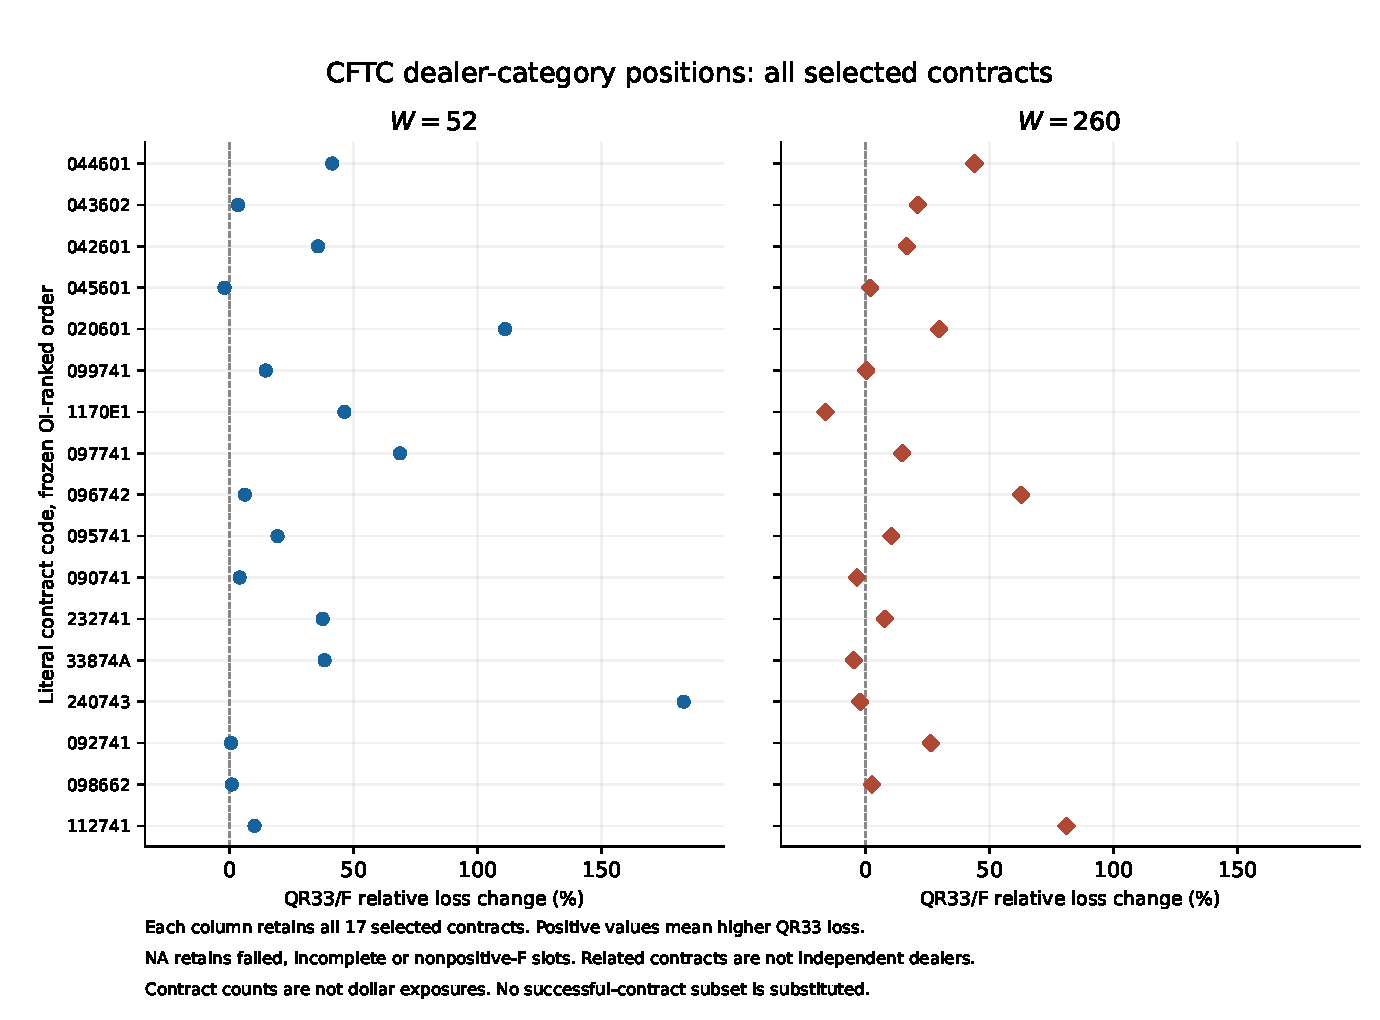
\includegraphics[width=.97\linewidth]{figures/v10-cftc-contract-changes.pdf}
\caption{Expanded-menu regression relative loss versus matched F for every eligible CFTC contract. Columns separate histories; code order follows the fixed open-interest ranking. Positive values mean higher regression loss.}\label{fig:v10-cftc}
\end{figure}

\subsubsection{Model confidence sets}

Joint comparison leaves matched historical methods alongside alternatives in most sets, with a single historical method surviving in only a small minority. These results support retaining historical controls while leaving many alternatives uneliminated under the fixed bootstrap approximation. Non-elimination does not establish equal predictive risk. Table~\ref{tab:v10-mcs-main} distinguishes literal membership from exact observed-loss equality. Supplement Section S31 retains every set, method p-value, equivalence class and prior unavailable method.

\begin{table}[t]\centering\small
\caption{Ninety-percent model confidence sets across all planned comparisons. Counts retain their own comparison or conditional-procedure denominators.}\label{tab:v10-mcs-main}
\begin{tabular}{lrrrrr}\toprule
Group & Complete & Matched $F/I$ & Sole literal $F/I$ & Conditional & Prior NA \\
 & / planned & included & & excluded & methods \\\midrule
FX original & 4/4 & 2/4 (50.0\%) & 0/4 (0.0\%) & 39/66 (59.1\%) & 6 \\
FX early2015 & 4/4 & 3/4 (75.0\%) & 0/4 (0.0\%) & 1/15 (6.7\%) & 2 \\
Treasury bills & 4/4 & 4/4 (100.0\%) & 0/4 (0.0\%) & 11/74 (14.9\%) & 4 \\
Other NYFed panels & 48/48 & 46/48 (95.8\%) & 0/48 (0.0\%) & 110/384 (28.6\%) & 48 \\
Same-record dailyFX & 4/4 & 4/4 (100.0\%) & 2/4 (50.0\%) & 5/8 (62.5\%) & 0 \\
CFTC & 34/34 & 31/34 (91.2\%) & 0/34 (0.0\%) & 31/136 (22.8\%) & 0 \\
All comparisons & 98/98 & 90/98 (91.8\%) & 2/98 (2.0\%) & 197/683 (28.8\%) & 60 \\
\bottomrule\end{tabular}
\par\smallskip\begin{minipage}{.98\linewidth}\footnotesize
All planned comparisons complete, so successful and planned denominators coincide. Matched F/I excludes rolling references and query-nearest state baselines. Conditional exclusions count complete procedure slots; prior NA methods are not statistical exclusions. A sole exact-loss class can retain several procedures: 4/98 sets have such a class containing F/I, versus 2/98 sole literal historical methods. Related tasks are not independent replications. The Supplement retains every set, p-value, loss class, secondary membership measure and availability record.
\end{minipage}\end{table}


\subsection{Scores and breach behavior answer different questions}

Accuracy rankings leave breach behavior unresolved: the matched FX gain coexists with more breaches before calibration (Table~\ref{tab:fx}). Pinball loss measures error amounts, while a strict-hit indicator records event occurrence. Monitoring reports should show both.

Elementary-score rankings cross for both original main comparisons (Supplement Figures S1--S2, Section S33). A separate 24-step FX comparison against rolling translated paths reverses near 20.6:1. Both six-step FX comparisons improve mean overrun and unused allowance. The weight reversal therefore belongs to the 24-step reference.

Loss and hit diagnostics answer different questions (Supplement Table S46, Section S33). HAC tests compare average loss; strict-hit tests examine event frequency and serial behavior. RMS-state diagnostics compare conditional predictive ability across training-defined groups \citep{gw2006}.

\FloatBarrier

\subsection{Isolating the penalty menu}\label{sec:extensions}

The weekly failures motivate a closer look at the penalty menu in calibrated simulations. Earlier stationary comparisons already produce large short-history regression losses. The fitted constant and switching arms use thirteen pre-evaluation weekly calibrations. The earlier stability screen rejects seven series pointwise and two after Holm correction. Supplement Sections S27--S28 retain the earlier calibrated simulations and stability diagnostics (Tables S27--S32).

The paired menu experiment changes only the ridge candidate menu and the stated exact-tie rule. It adds penalties one, ten and the intercept-only limit to full regression. Both regressions use the six-point menu. All paths, innovations, source calibrations and forecasting clocks match the earlier experiment. Thirty-two paired repetitions contribute to each complete source median. This isolates the executed menu comparison within these calibrated laws. The expanded procedure can choose ordinary I. Stronger finite penalties and access to I are not separately identified; near-parity loss alone supplies no evidence of added feature value.

The expanded full-regression medians move close to historical headroom in both arms (Table~\ref{tab:v10-menu-isolation}). Both arms improve in every source. The constant-arm near-parity prediction and the paired-improvement prediction hold. The switching-minus-constant difference misses the registered five-percentage-point increase. This outcome supports the menu explanation for these simulated losses; it leaves the empirical frequency mechanism unresolved.

\begin{table}[t]\centering\footnotesize
\setlength{\tabcolsep}{2pt}
\caption{Penalty-menu isolation on matched calibrated paths. Entries are the median relative loss (\%) across all 13 source medians, with the descriptive source IQR in brackets.}
\label{tab:v10-menu-isolation}
\begin{tabular}{lllrrr}\toprule
Arm & History & Regression & Original menu & Expanded menu & Missing sources \\
 & & & Median [IQR] & Median [IQR] & Original / expanded \\ \midrule
Constant & 52 & Full regression & \makebox[3.0em][r]{116.24} [\makebox[3.1em][r]{92.90}, \makebox[3.2em][r]{124.34}] & \makebox[3.0em][r]{0.21} [\makebox[3.1em][r]{-0.52}, \makebox[3.2em][r]{0.98}] & 0 / 0 \\
Constant & 52 & Four-feature & \makebox[3.0em][r]{-0.02} [\makebox[3.1em][r]{-1.55}, \makebox[3.2em][r]{1.73}] & \makebox[3.0em][r]{0.44} [\makebox[3.1em][r]{-1.69}, \makebox[3.2em][r]{1.90}] & 0 / 0 \\
Constant & 260 & Full regression & \textsc{NA} & \textsc{NA} & 1 / 1 \\
Constant & 260 & Four-feature & \makebox[3.0em][r]{-1.21} [\makebox[3.1em][r]{-1.69}, \makebox[3.2em][r]{-0.54}] & \makebox[3.0em][r]{-1.13} [\makebox[3.1em][r]{-1.69}, \makebox[3.2em][r]{-0.64}] & 0 / 0 \\
Switching & 52 & Full regression & \makebox[3.0em][r]{121.40} [\makebox[3.1em][r]{101.92}, \makebox[3.2em][r]{131.26}] & \makebox[3.0em][r]{-0.23} [\makebox[3.1em][r]{-1.88}, \makebox[3.2em][r]{0.98}] & 0 / 0 \\
Switching & 52 & Four-feature & \makebox[3.0em][r]{-0.03} [\makebox[3.1em][r]{-2.03}, \makebox[3.2em][r]{3.22}] & \makebox[3.0em][r]{0.38} [\makebox[3.1em][r]{-2.17}, \makebox[3.2em][r]{3.17}] & 0 / 0 \\
Switching & 260 & Full regression & \textsc{NA} & \textsc{NA} & 1 / 1 \\
Switching & 260 & Four-feature & \makebox[3.0em][r]{-0.27} [\makebox[3.1em][r]{-0.66}, \makebox[3.2em][r]{0.23}] & \makebox[3.0em][r]{-0.28} [\makebox[3.1em][r]{-0.75}, \makebox[3.2em][r]{0.48}] & 0 / 0 \\
\bottomrule\end{tabular}
\par\vspace{2pt}\begin{minipage}{.98\linewidth}\footnotesize
Each source median uses all 32 matched repetitions with relative loss $100(\overline L_{QR}/\overline L_F-1)$; positive values mean higher regression loss, and NA retains unavailable all-source summaries without substituting successful subsets.
Displays are rounded, while registered decisions use saved full-precision operands; full and four-feature regression correspond to QR33 and QR4.
The expanded four-feature exact-tie rule prefers stronger penalties, unlike its original rule; saved exact ties: 0, changed selections: 0.
\end{minipage}\end{table}


\begin{figure}[htbp]\centering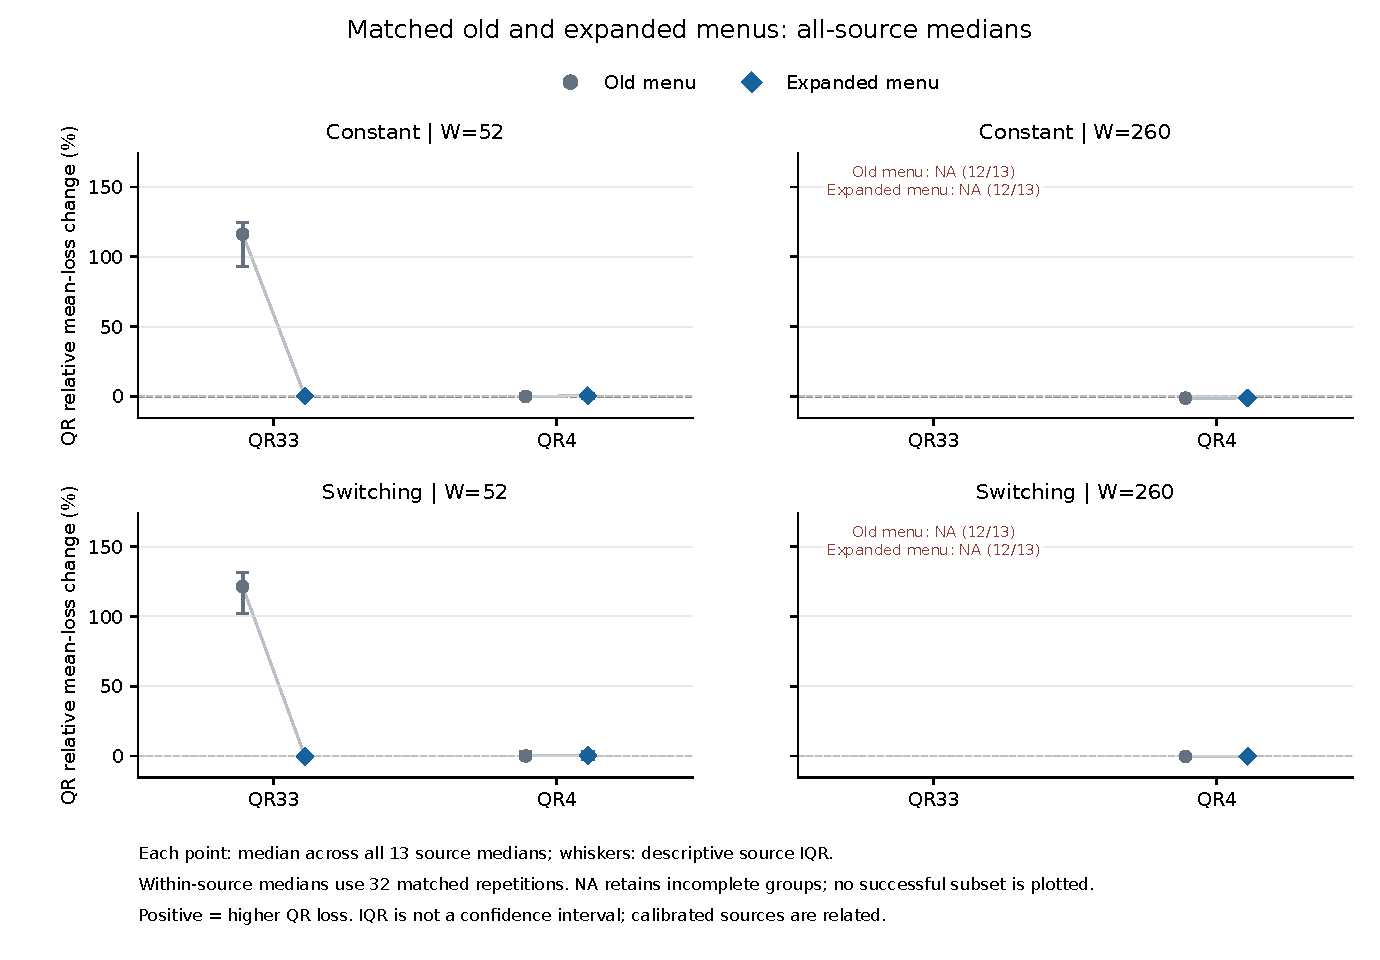
\includegraphics[width=.98\linewidth]{figures/v10-menu-isolation.pdf}
\caption{Paired penalty-menu isolation on unchanged calibrated paths. The expanded menu removes the large short-history full-regression loss in both arms. Longer-history full-regression summaries remain unavailable because a required repetition fails in each arm, with no successful-subset replacement.}\label{fig:mechanism}
\end{figure}

At history 260, one required full-regression repetition fails in each arm under the old low penalty. Both whole thirteen-source summaries remain unavailable. The experiment retains every failed cell and performs no retry. Earlier daily moment-qualification and hourly optimization failures also remain unavailable. Absence of a five-point switching increment is not evidence of equivalence.

\FloatBarrier

\section{RQ3: limit-cost regions}\label{sec:cost}

\[
J_m(\kappa,\beta,c)=\kappa\frac{\overline{C_m-B}}{m_F}
+\beta\,\overline{\mathbf 1\{Y>C_m\}}
+c\frac{\overline{(Y-C_m)_+}}{m_F},\qquad
m_F=\overline{C_F-B}>0,\quad\beta=b/m_F.
\]

For CFTC, higher reserve coefficients and lower fixed-breach coefficients generally favor expanded-menu regression over matched historical headroom, although the grid is not monotone (Figure~\ref{fig:v10-cost}).
At $c=1$, regression is strictly cheaper in $5/34$ comparisons at the sorted-grid centre $(\kappa,\beta)=(.1,.25)$, $32/34$ at $(1,0)$, and $1/34$ at the opposite corner $(.01,5)$.
These are illustrative costs, not observed operating costs; Supplement Section S32 gives the normalization, fixed grid and complete-method results.

\begin{figure}[p]\centering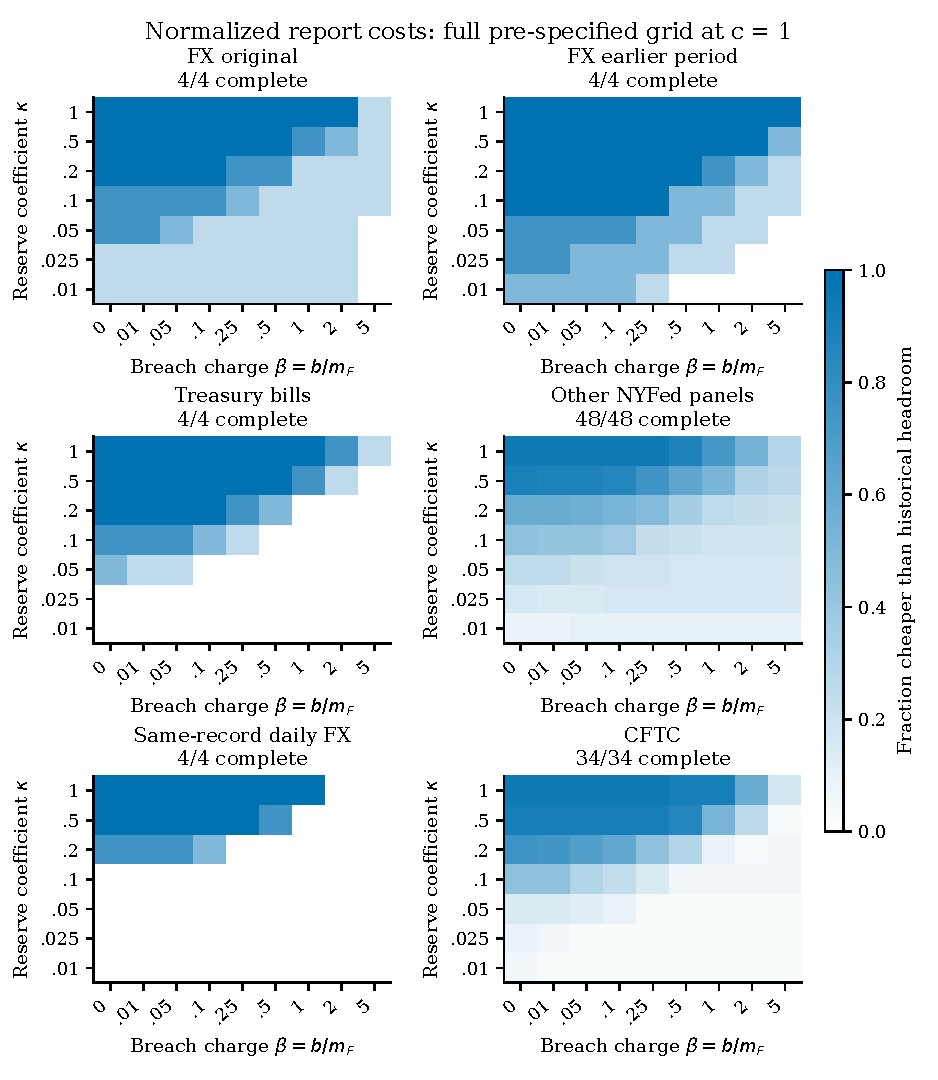
\includegraphics[width=.98\linewidth,height=.87\textheight,keepaspectratio]{figures/v10-cost-regions.pdf}
\caption{Fixed reserve and breach-charge regions with the exceedance coefficient held at unity. Color shows the fraction of related comparisons where the stated conditional procedure costs less than corrected historical headroom, with each source group retaining its own histories and horizons. These are descriptive fractions; all comparisons complete and the lower and upper fractions coincide.}\label{fig:v10-cost}
\end{figure}

\FloatBarrier

\section{Implications for model validation}\label{sec:implications}

\textbf{Benchmark against historical headroom.} Use the same completed labels, history length and refit schedule. Name the shorter rolling reference separately, since its FX ranking changes across periods.

\textbf{Retain corrected-rank history as a matched benchmark in these comparisons.} Expanded penalties reduce losses, while short-sample validation, including one-standard-error selection, still leaves large losses. The CFTC comparison also retains F/I in most model confidence sets. The ordinary empirical quantile is up to 36.5\% worse than corrected headroom in the earlier weekly grid.

\textbf{Report breaches with the score.} Show mean underprediction, mean unused headroom and strict-breach count on the same grid. The unwrapped matched FX gain and the daily regression exception both have more breaches than their historical references. Cost regions add reserve, breach-frequency and exceedance preferences to this joint evaluation.

\FloatBarrier

\section{Limitations}\label{sec:limitations}

The FX evidence describes a single market maker's client-flow record. Its original evaluation period was viewed before the conditional methods were specified. Rules for the earlier 2015 comparison followed the original results. The full-prefix backcast uses penalties selected after its issue dates and contains the earlier backcast. Its target paths were covered by previous scoring. Both exercises remain retrospective.

The New York Fed weekly categories share a reporting system and economic components; they are related aggregate tasks, not independent dealer replications. Treasury comparisons replay the downloaded economic-date vintage. Historical publication-time information is not reconstructed. Aggregation can offset gross dealer exposure; sampled net inventory also differs from settlement cash needs. Valuation and reporting-composition changes are not separated from trading. Sampled peaks omit intervening excursions. Daily last records also differ from verified closes or intraday maxima; the source timezone and release vintage are unknown.

Daily aggregation jointly changes physical histories, horizons, update cadence, calendar predictors, evaluation span and sampled targets. The same-record comparison leaves a pure frequency effect unidentified.

The design gives no causal interpretation or individual-predictor effects. The financial procedures provide no coverage guarantee under their dependence and calibration scheme. Trading and funding gains are not measured. Scoring weights are evaluation preferences, not estimated intervention or funding costs. Independent dealer records and prospective observations would broaden validation; finer exposure and cost data would connect reports to inventory actions.

Short overlapping validation samples and research-stage selection limit tuning stability and confirmatory inference. Longer weekly outer validation windows remain untested. The simulation designs use different menus, clocks, calibration laws and summary statistics. The paired menu experiment isolates that procedure change within the calibrated laws; empirical causation remains unresolved. The new parameter-switching process repeats fitted dwell lengths and adds artificial last-to-first transitions. Its stability screen uses a plug-in model-based approximation. Moment qualification and successful optimization leave the assumed law and boundary-estimate uncertainty unresolved. Failed cells and unavailable diagnostic comparisons retain those statuses.

CFTC categories provide an independent reporting system, not independent individual dealers. Full-history continuity creates a retrospective survivor universe. Open-interest ranking only orders the eligible contracts here. Conservative consolidation-family exclusions leave seventeen eligible contracts. Raw contracts have different exposure units; normalized comparisons do not recover common-dollar risks. Downloaded position dates omit actual historical first-release vintages and reporting delays. Two ingestion-schema clarifications followed acquisition but preceded every forecast and model-loss result; their original failed technical attempts remain documented.

Coefficients are fixed preferences; no estimated funding return, optimal intervention policy or trading-profit claim follows. The normalization uses evaluation-sample F headroom; ex ante institutional charges remain untested. MCS inference requires suitable loss dependence. The stationary bootstrap, modest samples and research-stage specification choices limit its nominal interpretation. Membership and cross-task fractions do not certify future coverage or simultaneous best-model status.

\FloatBarrier

\section{Conclusion}\label{sec:conclusion}

Historical rules are hard to beat. For RQ1, matched FX regression gains recur across periods, but rankings against the shorter rolling reference change. Delayed calibration preserves the later matched gain with a small breach-count difference. Matching history and update schedules is therefore central to interpreting conditional forecast gains.

For RQ2, historical controls remain competitive in related weekly categories, same-record daily aggregates and the independent CFTC reporting system. They usually remain in model confidence sets alongside alternatives. Short-sample validation still fails to protect the historical benchmark consistently. The calibrated paired experiment brings full regression near its historical reference by expanding the penalty menu. The registered switching increment is unsupported, while the empirical low-frequency mechanism remains unidentified.

For RQ3, higher reserve charges and lower fixed breach charges generally favor expanded regression in CFTC, with local exceptions. Lower forecast scores therefore need not imply lower limit costs. Validation should report reserve amounts, breach counts and exceedance amounts together, using the cost regions in Figure~\ref{fig:v10-cost}.

\FloatBarrier

\section*{Data and code availability}
\paragraph{Data availability.} The FX input is the specified version of the Kaggle Net Position Time Series Dataset. The owning metadata labels its license ``Data files \copyright\ Original Authors.'' This repository supplies the acquisition route and input fingerprint, but excludes raw FX observations and private per-issue prediction vectors. Obtain the source from \url{https://www.kaggle.com/datasets/davidlindsay1979/net-position-time-series-dataset} subject to the original rights holders' terms.

The New York Fed aggregates are available from its Primary Dealer Statistics service under the Bank's Terms of Use. The repository preserves the unchanged accepted Treasury snapshot with attribution and identifies study calculations separately. Copying or distributing that content remains subject to its source notices, attribution, modification labelling, continuing conditions and endorsement restrictions: \url{https://www.newyorkfed.org/privacy/termsofuse.html}. The code license does not replace those source conditions.

The CFTC application uses the public TFF historical files from \url{https://www.cftc.gov/MarketReports/CommitmentsofTraders/HistoricalCompressed/index.htm}. The repository includes unchanged downloaded archives and a per-file URL, acquisition time, byte count and SHA-256 record in \texttt{data/cftc-tff/provenance.json}.

\paragraph{Code availability.} Code, saved results and version-specific reproduction instructions are available at \url{https://github.com/ByronLi0207/financial-mathematics-paper-20261020/tree/revision-v10b}. The v10 package adds paired menu isolation, official CFTC sources, full MCS results and fixed cost regions. Earlier results remain unchanged in their versioned directories. Document compilation and restricted-input financial replay have separate instructions. Complete, adverse, failed and unavailable outcomes are retained.

\section*{Author-provided information}
Author information: [TO BE COMPLETED BY AUTHOR].\par
ORCID: [TO BE COMPLETED BY AUTHOR].\par
Funding: [TO BE COMPLETED BY AUTHOR].\par
Competing interests: [TO BE COMPLETED BY AUTHOR].\par
AI statement: [TO BE COMPLETED BY AUTHOR].

\begin{thebibliography}{99}
\raggedright
\bibitem[Arjani et al.(2020)]{arjani2020} Arjani, N., Li, F., \& Sabetti, L. (2020). \emph{Monitoring intraday liquidity risks in a real time gross settlement system}. Payments Canada. \url{https://www.payments.ca/sites/default/files/discussion_paper_monitoring_intraday_liquidity_risks_in_a_real_time_gross_settlement_system.pdf}.

\bibitem[Avellaneda \& Stoikov(2008)]{avellaneda2008} Avellaneda, M., \& Stoikov, S. (2008). High-frequency trading in a limit order book. \emph{Quantitative Finance}, \emph{8}(3), 217--224. \url{https://doi.org/10.1080/14697680701381228}.

\bibitem[Barone-Adesi et al.(1999)]{barone1999} Barone-Adesi, G., Giannopoulos, K., \& Vosper, L. (1999). VaR without correlations for portfolios of derivative securities. \emph{Journal of Futures Markets}, \emph{19}(5), 583--602. \url{https://doi.org/10.1002/(SICI)1096-9934(199908)19:5<583::AID-FUT5>3.0.CO;2-S}.

\bibitem[Board of Governors of the Federal Reserve System(2013)]{fr2004_2013} Board of Governors of the Federal Reserve System (2013, March). \emph{Reporting guidelines for preparing the FR 2004 primary government securities dealers reports}. Board of Governors of the Federal Reserve System. \url{https://www.federalreserve.gov/apps/reportingforms/Download/DownloadAttachment?guid=f555fe11-e149-479b-8088-4ed4e9ae1206}.

\bibitem[Board of Governors of the Federal Reserve System(2024)]{fr2004_2024} Board of Governors of the Federal Reserve System (2024, July). \emph{Instructions for the preparation of government securities dealers reports: Reporting form FR 2004}. Board of Governors of the Federal Reserve System. \url{https://www.federalreserve.gov/apps/reportingforms/Download/DownloadAttachment?guid=950ab256-b485-4586-99b0-b27eb205fdfa}.

\bibitem[Bollerslev(1986)]{bollerslev1986} Bollerslev, T. (1986). Generalized autoregressive conditional heteroskedasticity. \emph{Journal of Econometrics}, \emph{31}(3), 307--327. \url{https://doi.org/10.1016/0304-4076(86)90063-1}.

\bibitem[Boudoukh et al.(2004)]{boudoukh2004} Boudoukh, J., Richardson, M., Stanton, R., \& Whitelaw, R. F. (2004). MaxVaR: Long-horizon value at risk in a mark-to-market environment. \emph{Journal of Investment Management}, \emph{2}(3), 1--6. \url{https://pages.stern.nyu.edu/~rwhitela/papers/maxvar%20joim04.pdf}.

\bibitem[Christoffersen(1998)]{christ1998} Christoffersen, P. F. (1998). Evaluating interval forecasts. \emph{International Economic Review}, \emph{39}(4), 841--862. \url{https://doi.org/10.2307/2527341}.

\bibitem[Commodity Futures Trading Commission(n.d.)]{cftcTFF} Commodity Futures Trading Commission (n.d.). \emph{Traders in financial futures: Historical compressed reports}. \url{https://www.cftc.gov/MarketReports/CommitmentsofTraders/HistoricalCompressed/index.htm}. Retrieved October 24, 2026.

\bibitem[Diebold \& Mariano(1995)]{dm1995} Diebold, F. X., \& Mariano, R. S. (1995). Comparing predictive accuracy. \emph{Journal of Business \& Economic Statistics}, \emph{13}(3), 253--263. \url{https://doi.org/10.1080/07350015.1995.10524599}.

\bibitem[Duffie et al.(2023)]{duffie2023} Duffie, D., Fleming, M. J., Keane, F. M., Nelson, C., Shachar, O., \& Van Tassel, P. (2023). \emph{Dealer capacity and U.S. Treasury market functionality} (Staff Report No. 1070, August; revised October). Federal Reserve Bank of New York Staff Reports. \url{https://doi.org/10.59576/sr.1070}.

\bibitem[Ehm et al.(2016)]{ehm2016} Ehm, W., Gneiting, T., Jordan, A., \& Krüger, F. (2016). Of quantiles and expectiles: Consistent scoring functions, Choquet representations and forecast rankings. \emph{Journal of the Royal Statistical Society Series B: Statistical Methodology}, \emph{78}(3), 505--562. \url{https://doi.org/10.1111/rssb.12154}.

\bibitem[Engle \& Manganelli(2004)]{engle2004} Engle, R. F., \& Manganelli, S. (2004). CAViaR: Conditional autoregressive value at risk by regression quantiles. \emph{Journal of Business \& Economic Statistics}, \emph{22}(4), 367--381. \url{https://doi.org/10.1198/073500104000000370}.

\bibitem[Federal Reserve Bank of New York(n.d.)]{nyfeddata} Federal Reserve Bank of New York (n.d.). \emph{Primary dealer statistics} [Data set]. Federal Reserve Bank of New York. \url{https://www.newyorkfed.org/markets/counterparties/primary-dealers-statistics}. Retrieved October 23, 2026.

\bibitem[Giacomini \& White(2006)]{gw2006} Giacomini, R., \& White, H. (2006). Tests of conditional predictive ability. \emph{Econometrica}, \emph{74}(6), 1545--1578. \url{https://doi.org/10.1111/j.1468-0262.2006.00718.x}.

\bibitem[Gibbs \& Candès(2021)]{gibbs2021} Gibbs, I., \& Candès, E. J. (2021). Adaptive conformal inference under distribution shift. \emph{Advances in Neural Information Processing Systems}, \emph{34}, 1660--1672. \url{https://proceedings.neurips.cc/paper_files/paper/2021/hash/0d441de75945e5acbc865406fc9a2559-Abstract.html}.

\bibitem[Gneiting(2011)]{gneiting2011} Gneiting, T. (2011). Making and evaluating point forecasts. \emph{Journal of the American Statistical Association}, \emph{106}(494), 746--762. \url{https://doi.org/10.1198/jasa.2011.r10138}.

\bibitem[Hansen(1992)]{hansen1992} Hansen, B. E. (1992). Testing for parameter instability in linear models. \emph{Journal of Policy Modeling}, \emph{14}(4), 517--533. \url{https://doi.org/10.1016/0161-8938(92)90019-9}.

\bibitem[Hansen et al.(2011)]{mcs2011} Hansen, P. R., Lunde, A., \& Nason, J. M. (2011). The model confidence set. \emph{Econometrica}, \emph{79}(2), 453--497. \url{https://doi.org/10.3982/ECTA5771}.


\raggedright

\bibitem[Harvey et al.(1997)]{hln1997} Harvey, D., Leybourne, S., \& Newbold, P. (1997). Testing the equality of prediction mean squared errors. \emph{International Journal of Forecasting}, \emph{13}(2), 281--291. \url{https://doi.org/10.1016/s0169-2070(96)00719-4}.

\bibitem[Hastie et al.(2009)]{hastie2009} Hastie, T., Tibshirani, R., \& Friedman, J. (2009). \emph{The elements of statistical learning: Data mining, inference, and prediction} (2nd ed.). Springer. \url{https://doi.org/10.1007/978-0-387-84858-7}.

\bibitem[Holm(1979)]{holm1979} Holm, S. (1979). A simple sequentially rejective multiple test procedure. \emph{Scandinavian Journal of Statistics}, \emph{6}(2), 65--70. \url{https://www.jstor.org/stable/4615733}.

\bibitem[Hull \& White(1998)]{hull1998} Hull, J., \& White, A. (1998). Incorporating volatility updating into the historical simulation method for value-at-risk. \emph{The Journal of Risk}, \emph{1}(1), 5--19. \url{https://doi.org/10.21314/jor.1998.001}.

\bibitem[Koenker \& Bassett(1978)]{koenker1978} Koenker, R., \& Bassett, G., Jr. (1978). Regression quantiles. \emph{Econometrica}, \emph{46}(1), 33--50. \url{https://doi.org/10.2307/1913643}.

\bibitem[Kupiec(1995)]{kupiec1995} Kupiec, P. H. (1995). Techniques for verifying the accuracy of risk measurement models. \emph{The Journal of Derivatives}, \emph{3}(2), 73--84. \url{https://doi.org/10.3905/jod.1995.407942}.

\bibitem[Lindsay(2020)]{dataset} Lindsay, D. (2020). \emph{Net position time series dataset} (Version 2) [Data set]. Kaggle. \url{https://www.kaggle.com/datasets/davidlindsay1979/net-position-time-series-dataset}.

\bibitem[McNeil \& Frey(2000)]{mcneilfrey2000} McNeil, A. J., \& Frey, R. (2000). Estimation of tail-related risk measures for heteroscedastic financial time series: An extreme value approach. \emph{Journal of Empirical Finance}, \emph{7}(3--4), 271--300. \url{https://doi.org/10.1016/s0927-5398(00)00012-8}.

\bibitem[Meinshausen(2006)]{meinshausen2006} Meinshausen, N. (2006). Quantile regression forests. \emph{Journal of Machine Learning Research}, \emph{7}(35), 983--999. \url{https://www.jmlr.org/papers/v7/meinshausen06a.html}.

\bibitem[Newey \& West(1987)]{nw1987} Newey, W. K., \& West, K. D. (1987). A simple, positive semi-definite, heteroskedasticity and autocorrelation consistent covariance matrix. \emph{Econometrica}, \emph{55}(3), 703--708. \url{https://doi.org/10.2307/1913610}.

\bibitem[Petrunia et al.(2019)]{petrunia2019} Petrunia, R., Sabetti, L., \& Voia, M. (2019). \emph{Tail risk in the automated clearing settlement system (ACSS)} (Discussion Paper No. 7). Payments Canada. \url{https://www.payments.ca/sites/default/files/tail_risk_in_the_automated_clearing_settlement_system_acss.pdf}.

\bibitem[Sussman(2023)]{sussman2023} Sussman, E. (2023). A strengthened Orlicz--Pettis theorem via Itô--Nisio. \emph{Annals of Functional Analysis}, \emph{14}(1), Article 22. \url{https://doi.org/10.1007/s43034-022-00225-1}.

\bibitem[van den Hoogen(2017)]{hoogen2017} van den Hoogen, S. (2017). \emph{Intraday liquidity risk estimation using transaction data: An extreme value theory approach} [Master's thesis, Delft University of Technology]. \url{https://resolver.tudelft.nl/uuid:1c0c4545-bb07-4916-aa37-1d4bea3b7872}.

\bibitem[Wisniewski et al.(2020)]{wisniewski2020} Wisniewski, W., Lindsay, D., \& Lindsay, S. (2020). Application of conformal prediction interval estimations to market makers' net positions. In \emph{Proceedings of the Ninth Symposium on Conformal and Probabilistic Prediction and Applications} (Proceedings of Machine Learning Research, Vol. 128, pp. 285--301). \url{https://proceedings.mlr.press/v128/wisniewski20a.html}.

\bibitem[Wisniewski(2024)]{wisniewski2024} Wisniewski, W. J. (2024). \emph{Net position and retail trader behaviour: Implications for market makers' risk management strategies} [Doctoral thesis, Royal Holloway, University of London]. \url{https://pure.royalholloway.ac.uk/en/publications/net-position-and-retail-trader-behaviour-implications-for-market-/}.
\end{thebibliography}

\end{document}
